\documentclass[tikz,border=10pt]{standalone}
\usepackage{amsmath}
\usetikzlibrary{arrows.meta, positioning, calc, fit, decorations.pathreplacing}

\definecolor{c1}{HTML}{000000}  % black       - structure, axes
\definecolor{c2}{HTML}{233D4D}  % deep slate  - tokens and rows
\definecolor{c3}{HTML}{FE7F2D}  % orange      - the measurements themselves
\definecolor{c4}{HTML}{EAECF0}  % cool grey   - panel fills
\definecolor{axiscolor}{HTML}{333333}
\definecolor{labelcolor}{HTML}{5F6B75}

\begin{document}
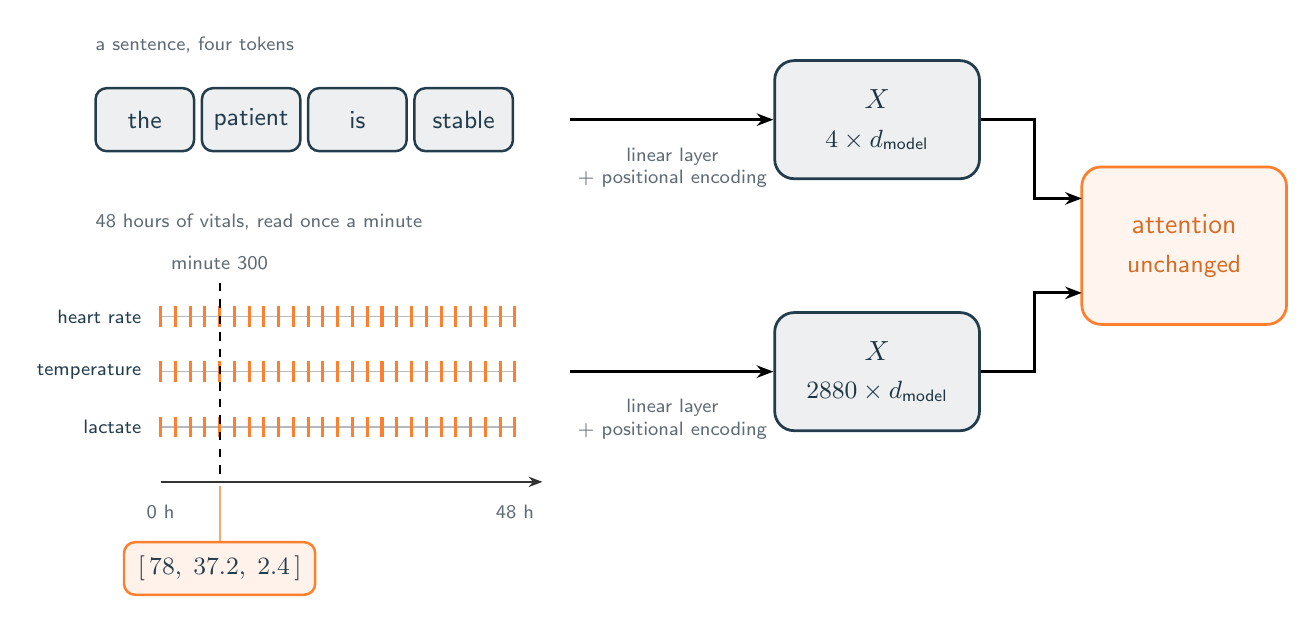
\begin{tikzpicture}[
    every node/.style={font=\sffamily},
    tok/.style={
        rectangle, rounded corners=4pt, minimum width=1.25cm,
        minimum height=0.8cm, line width=0.9pt,
        draw=c2, fill=c2!8, text=c2, font=\sffamily\small,
    },
    block/.style={
        rectangle, rounded corners=7pt, minimum width=2.6cm,
        minimum height=1.5cm, line width=1.0pt,
        draw=#1, fill=#1!8, text=#1!85!black, align=center,
    },
    arr/.style={-{Stealth[length=6pt]}, line width=1.1pt, color=#1},
    lab/.style={font=\sffamily\scriptsize, text=labelcolor},
    chan/.style={font=\sffamily\scriptsize, text=c2, anchor=east},
]

% ---------------------------------------------------------------- lane A
\node[lab, anchor=west] at (-0.05, 4.40) {a sentence, four tokens};
\node[tok] at (0.70, 3.45) {the};
\node[tok] at (2.05, 3.45) {patient};
\node[tok] at (3.40, 3.45) {is};
\node[tok] at (4.75, 3.45) {stable};

% ---------------------------------------------------------------- lane B
\node[lab, anchor=west] at (-0.05, 2.15) {48 hours of vitals, read once a minute};

\foreach \y/\name in {0.95/heart rate, 0.25/temperature, -0.45/lactate}{
    \node[chan] at (0.78, \y) {\name};
    \draw[c2!35, line width=0.6pt] (0.90, \y) -- (5.40, \y);
    \foreach \i in {0,...,24}{
        \draw[c3, line width=1.1pt]
            ($(0.90, \y) + (\i*0.1875, -0.13)$) -- ($(0.90, \y) + (\i*0.1875, 0.13)$);
    }
}

% time axis
\draw[axiscolor, line width=0.8pt, -{Stealth[length=5pt]}] (0.90, -1.15) -- (5.75, -1.15);
\node[lab, anchor=north] at (0.90, -1.32) {0 h};
\node[lab, anchor=north] at (5.40, -1.32) {48 h};

% the highlighted minute
\node[lab, anchor=south] at (1.65, 1.42) {minute 300};
\draw[c1, line width=0.8pt, dashed] (1.65, 1.38) -- (1.65, -1.15);
\node[
    rectangle, rounded corners=4pt, draw=c3, fill=c3!10, text=c2,
    line width=0.9pt, font=\sffamily\small, inner sep=5pt
] (triple) at (1.65, -2.25) {$[\,78,\; 37.2,\; 2.4\,]$};
\draw[c3!70, line width=0.8pt] (1.65, -1.20) -- (triple.north);

% ---------------------------------------------------------------- X blocks
\node[block=c2] (xa) at (10.00, 3.45) {$X$\\[2pt] \small $4 \times d_{\text{model}}$};
\node[block=c2] (xb) at (10.00, 0.25) {$X$\\[2pt] \small $2880 \times d_{\text{model}}$};

\draw[arr=c1] (6.10, 3.45) -- (xa.west);
\draw[arr=c1] (6.10, 0.25) -- (xb.west);

\node[lab, anchor=north, align=center] at (7.40, 3.22)
    {linear layer\\ $+$ positional encoding};
\node[lab, anchor=north, align=center] at (7.40, 0.02)
    {linear layer\\ $+$ positional encoding};

% ---------------------------------------------------------------- attention
\node[block=c3, minimum height=2.0cm] (att) at (13.90, 1.85)
    {attention\\[2pt] \small unchanged};

\draw[arr=c1] (xa.east) -- (12.00, 3.45) -- (12.00, 2.45) -- (12.60, 2.45);
\draw[arr=c1] (xb.east) -- (12.00, 0.25) -- (12.00, 1.25) -- (12.60, 1.25);

\end{tikzpicture}
\end{document}
